\documentclass[12pt]{article}
%\documentclass{elsart}
%%\bibliographystyle{elsevier}
\usepackage{fancyhdr}
\topmargin -0.3in
\headheight 0.0in
\headsep 0.5in
\textheight 9.4in
\oddsidemargin -.0in
\evensidemargin -.0in
\textwidth 6.6in
\renewcommand{\baselinestretch}{1.4}
\usepackage{epsfig}
\input epsf
\usepackage[dvips]{color}
\usepackage{lscape}
\usepackage{longtable}
%
\def\beqn{\begin{eqnarray}}
\def\eeqn{\end{eqnarray}}
\def\beq{\begin{equation}}
\def\eeq{\end{equation}}

\pagenumbering{arabic}	




\newcommand{\la}{\langle}
\newcommand{\ra}{\rangle}
\newcommand{\zh}{z}
\newcommand{\xbj}{x_{\scriptscriptstyle B}}
%
\newcommand{\thp}{$\Theta^+$ }
\newcommand{\Thgg}{$\theta_{\gamma^*\gamma}~$}
\newcommand{\Phgg}{$\phi_{\gamma^*\gamma}~$}
\newcommand{\Epg}{$ep~\rightarrow~ep\gamma~$}
\newcommand{\Eppiz}{$ep~\rightarrow~ep\pi^0~$}
\newcommand{\Enpip}{$ep~\rightarrow~en\pi^+~$}
\newcommand{\EppiD}{$ep~\rightarrow~e\pi \Delta~$}
\newcommand{\Epeta}{$ep~\rightarrow~ep\eta~$}
\newcommand{\Epr}{$ep~\rightarrow~ep\rho~$}
\newcommand{\EpX}{$ep~\rightarrow~epX~$}
\newcommand{\EpKY}{$ep~\rightarrow~eKY~$}
\newcommand{\vEpg}{$\vec ep~\rightarrow~ep\gamma~$}
\def\gevc2{(GeV/c)$^2$}
\newcommand*{\jlab}{Jefferson Lab, Newport News, VA 23606, USA}
\newcommand*{\yerevan}{Yerevan Physics Institute, 375036 Yerevan, Armenia}
\newcommand*{\frascati}{Istituto Nazionale di Fisica Nucleare, Laboratori Nazionali di Frascati, P.O. 13, 00044 Frascati, Italy}
\newcommand*{\genova}{Istituto Nazionale di Fisica Nucleare, Sezione di Genova
 e Dipartimento di Fisica dell'Universita, 16146 Genova, Italy}
\newcommand*{\ipn}{Institut de Physique Nucleaire d'Orsay, IN2P3, BP 1, 91406 Orsay, France}
\newcommand*{\uvch}{University of Virginia, Department of Physics, Charlottesville, VA 22903, USA}
\newcommand*{\nsuva}{Norfolk State University, Norfolk VA 23504, USA}
\newcommand*{\rpi}{Rensselaer Polytechnic Institute, Department of Physics, Troy, NY 12181, USA}
\newcommand*{\moscow}{Moscow  State University, 11989 Moscow, Russia}
\newcommand*{\ucla}{University of California at Los Angeles, Department of Physics and 
Astronomy, Los Angeles, CA 90095-1547, USA}
\newcommand*{\ohio}{Ohio University, Department of Physics, Athens, OH 45701, USA}
\newcommand*{\gwu} {Center for Nuclear Studies,
The George Washington University, Washington, D.C., 20052}
\newcommand*{\jmu} {James Madison University, Harrisonburg, Virginia
22807, USA}




%
%%%%%%%%%%%%%%%%%%%%%%%%%%%%%%%%%%%%%%%%%%%%%%%%%%%%%%
%

%

\begin{document}


\thispagestyle{empty}
\begin{center}
{\Huge \bf Pre-shower calorimeter for the CLAS12 detector}
\end{center}
\vspace{2cm}
\begin{figure}[ht]
\begin{center}
\vspace{1cm}
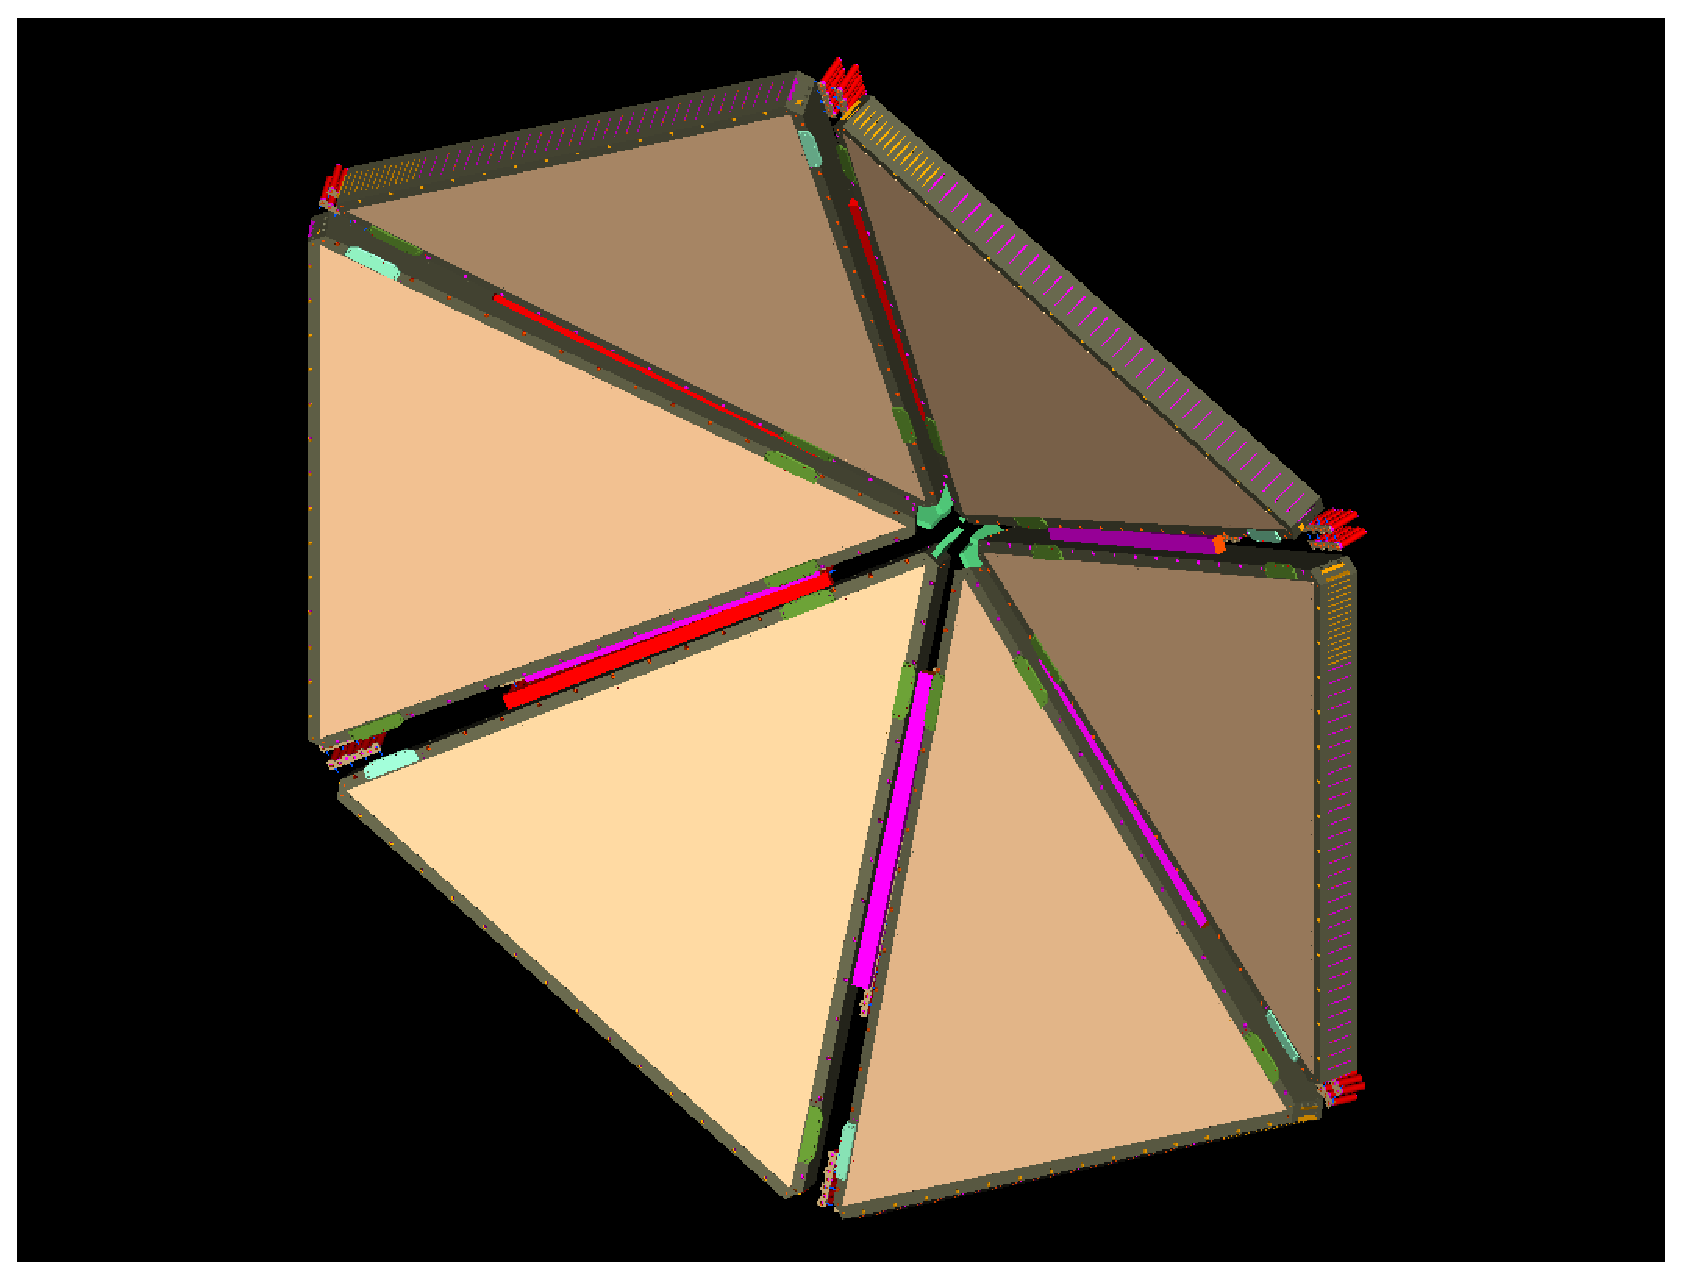
\epsfig{file=pcal_all_6.eps,width=14cm}
\end{center}
\end{figure}

\begin{center}
\Large Version 1.1
\end{center}


\pagestyle{empty}

\thispagestyle{empty}

\begin{center}
\title{Pre-shower calorimeter for the CLAS12 detector}
\date{}


%\vskip 0.7cm
\maketitle

{\it{G. Asryan, N. Dashyan, H. Voskanyan \\}}
\smallskip
{\small{\yerevan}}
\bigskip

{\it{V. Burkert, D. Kashy, S. Stepanyan \\}}
\smallskip
{\small{\jlab}}
\bigskip

\vskip 0.4cm
{\it{M. MacCormick, P. Rosier \\}}
\smallskip
{\small{\ipn}}
\bigskip

\vskip 0.4cm
{\it{C. Salgado, M. Khandaker\\}}
\smallskip
{\small{\nsuva}}
\bigskip


{\it K. Hicks\\}
\smallskip
{\small \ohio}
\bigskip

{\it K. Giovanetti\\}
\smallskip
{\small \jmu}
%\bigskip



\end{center}






\thispagestyle{empty}

\begin{abstract}

The CLAS12 detector package will include the existing electromagnetic
calorimeters of the CLAS detector. Calorimeters in
CLAS12 will be used primarily for identification of electrons,
photons, $\pi^0\to \gamma\gamma$, and
neutrons. At high energies, the existing calorimeters alone will not be
able to provide necessary accuracy for energy and position measurements
of electromagnetic showers. Therefore, pre-shower calorimeters are
proposed to install in front of the existing electromagnetic
calorimeters. The pre-shower calorimeter will have similar geometrical design and
the readout scheme as the present calorimeters: lead-scintillator
sandwich with three stereo readout planes. Proposed pre-shower will
be about $5.5$ radiation 
lengths and will have smaller readout segmentation in the
transverse direction than the present calorimeter. Light, produced in the scintillator strips will
be transported to a photomultiplier tube via 1 mm diameter wave-length
shifting fibers, embedded in the surface of the strip. This addition
to the CLAS12 electromagnetic calorimetry in the forward region will
allow accurate determination of the shower energy
and separation of close clusters from high energy $\pi^0$ decays for
energies up to $10$ GeV. 

\end{abstract}

\newpage
\tableofcontents

\newpage

\fancypagestyle{myheading}{%                % Redefining plain style
\fancyhf{} % clear all header and footer fields
\fancyhead[C]{\vspace{0.5cm}\line(1,0){500}\vspace{-0.5cm}}
\fancyhead[l]{\mbox{\bfseries CLAS12 Technical Design Report}}
\fancyhead[r]{\mbox{\bfseries Version 1.1 \date{\today}}}
\fancyfoot[C]{\mbox{\bfseries  \thepage }}
\fancyfoot[r]{\mbox{\bfseries Pre-shower calorimeter}}
\fancyfoot[l]{\vspace{-1cm}\line(1,0){500}}
}
\renewcommand{\headrulewidth}{0pt}
\renewcommand{\footrulewidth}{0pt}
\pagestyle{myheading}

\section{Overview and Physics Requirements}

The primary goal of experiments using the {\tt CLAS12} detector at energies
up to 11~GeV is the study of internal nucleon dynamics by accessing the 
nucleon's generalized parton distributions (GPDs).  This is accomplished 
through the measurement of deeply virtual Compton scattering (DVCS), deeply 
virtual meson production (DVMP), and single spin asymmetries (SSA). Towards 
this end, the detector has been tuned for studies of exclusive and 
semi-inclusive reactions in a wide kinematic range. 

The {\tt CLAS12} program of experiments goes further than just GPDs and 
includes experiments such as the space-time characteristics of 
hadronization. Detection of $\pi^0$s and $K^0$s is important to 
complement the measurements of nuclear attenuation seen for charged pions
and kaons.  These experiments depend on the ability to detect neutral and
charged pions at high momentum.

Copious amounts of high-energy particles, both charged and neutral, will be 
produced at experiments to be done at {\tt CLAS12}.  Electromagnetic
calorimeters for the {\tt CLAS12} detector should have sufficient radiation
length to absorb the full energy of the electromagnetic showers produced by 
high-energy electrons and photons.  High-energy neutral pions present a 
challenge as well, as they decay immediately into two photons with an 
opening angle that decreases as the $\pi^0$ momentum increases.  Unless 
there is sufficient position resolution in the electromagnetic calorimeter 
of the {\tt CLAS12} detector, the two photons from $\pi^0$ decay could be 
seen as a single high-energy photon.

The separation of single high-energy photons from the photons of $\pi^0$ 
decay is very important to the deeply virtual Compton scattering (DVCS) 
experiments that represents a major physics program planned for {\tt CLAS12}.
A single high-energy photon is produced in the reaction $ep \to ep\gamma$
and the largest background to this process is from single $\pi^0$ 
production, $ep \to ep\pi^0$.  Clearly, good $\pi^0$ detection is crucial 
to separate these two processes.  In addition, direct $\pi^0$ production 
complements the DVCS measurements by accessing GPDs at low and high 
momentum transfer $|t|$.

Simulations have shown that the existing electromagnetic calorimeter (EC)
of {\tt CLAS}~\cite{ec} will not be able to absorb the full energy of the
electromagnetic showers produced by electrons and photons with momenta 
above 5~GeV.  The leakage from the back of the calorimeter will diminish 
the energy resolution, see Fig.~\ref{fig:ecsim}a.  For the simple 
kinematics of $\pi^0$ decay, above a momentum of 5.5~GeV the opening angle 
of the decay photons becomes too small to be resolved with the existing 
EC system, which is at a distance of about 6~m from the target.  The readout 
segmentation of the EC is only $\sim$10~cm.  Simulations with the GEANT 
software for the {\tt CLAS12} geometry show that these pions would be seen 
as a single cluster (i.e., one photon) by the event reconstruction 
software, see Fig.~\ref{fig:ecsim}b.

%%%%%%%%%%%%%%%%%%%%%%%%%%%%%%%%%%%%%%%%%%%%%%%%%%%%%%%%%%%%%%%%%%%%%%%%%
\begin{figure}[ht]
\vspace{70mm}
\special{psfile=../preshower/ecres.eps hscale=45 vscale=45 hoffset=30 
voffset=-15}
\special{psfile=../preshower/2clusteff.eps hscale=45 vscale=45 hoffset=245 
voffset=-15}
\mbox{
\begin{picture}(-10,-10)(350,0)
\put(520,170){\large {\bf (a)}}
\put(740,170){\large {\bf (b)}}
\end{picture}}
\caption{\small{Performance of the EC at high energies. a) The energy 
resolution of the EC as a function of the inverse square root of energy. 
b) The efficiency of reconstruction of two clusters from $\pi^0$ decay
photons as a function of pion momentum, filled red squares.  The open
symbols correspond to the probability that a single cluster is 
reconstructed with the same energy as the simulated pion.}} 
\label{fig:ecsim} 
\end{figure}
%%%%%%%%%%%%%%%%%%%%%%%%%%%%%%%%%%%%%%%%%%%%%%%%%%%%%%%%%%%%%%%%%%%%%%%%%

To reconstruct the energy of high-energy showering particles and to
separate high-energy $\pi^0$s and photons, a pre-shower detector (PCAL), 
with finer granularity, will be built and installed in front of the 
current EC.  The PCAL will have a similar geometry as the current EC.  It 
will consist of a lead-scintillator sandwich with three stereo readout planes. 
Initial simulations have shown~\cite{natalia,whitlow} that 15 layers of 
1-cm thick scintillator layers, segmented into 4.5-cm wide strips, 
sandwiched between lead sheets of 2.2-mm thickness, corresponds to about 
5.5 radiation lengths, and will be sufficient to address issues arising at 
high energies.

In summary, accurate reconstruction of high-energy electromagnetic showers 
and detection of $\pi^0$s, and in particular the ability to distinguish 
single high-energy photons from the two-photon clusters from $\pi^0$ decay, 
is essential to the experimental program using the {\tt CLAS12} detector at 
high energies that will be part of the GPD program.  Efficient detection of 
high-momentum $\pi^0$s is also needed for a variety of other {\tt CLAS12} 
proposals.  The physics dictates the need for a pre-shower calorimeter to 
be placed in front of the existing EC.  Simulations show that good $\pi^0$ 
identification can be obtained with full coverage of the EC front surface. 
In addition to the improved performance in the reconstruction of 
electromagnetic showers, the increase of the overall scintillator thickness 
in the {\tt CLAS12} forward electromagnetic calorimeters will increase the 
detection efficiency for neutrons. 



\section{Conceptual Design}

The design parameters of the PCAL were established using the full GEANT 
simulations of the PCAL-EC system.  As a tool, a modified GEANT simulation 
computer program for the {\tt CLAS} detector was used.  The PCAL was 
positioned in front of the current EC as shown in Fig.~\ref{fig:clas12fwd}.  
These studies are described in detail in Refs.~\cite{natalia,whitlow} and are 
summarized below.  The mechanical design depends on the number of 
scintillator-lead layers, on the angular coverage of the PCAL, and on the 
size of the readout segmentation.  These parameters were determined by the 
physics requirements for the detection and identification of high-energy 
electrons, photons, and $\pi^0$s via $2\gamma$ decay.  

%%%%%%%%%%%%%%%%%%%%%%%%%%%%%%%%%%%%%%%%%%%%%%%%%%%%%%%%%%%%%%%%%%%%%%%%%
\begin{figure}[ht]
\vspace{100mm}
\special{psfile=../preshower/clas12fwd.epsi hscale=55 vscale=50 hoffset=70 
voffset=-60}
\caption{\small{Particle ID detector package of the {\tt CLAS12} forward
region.  The low threshold {\v C}erenkov counter is shown in magenta, two
layers of FTOF counters are shown in green and yellow, the PCAL is shown 
in red, and the EC in blue.}}  
\label{fig:clas12fwd} 
\end{figure}
%%%%%%%%%%%%%%%%%%%%%%%%%%%%%%%%%%%%%%%%%%%%%%%%%%%%%%%%%%%%%%%%%%%%%%%%%

Initial simulations were carried out with 15 layers of lead and 
scintillator (similar to the inner part of the EC), using 35-mm wide 
segmentation for the scintillator layers, corresponding to about 108 
readout channels in each stereo view.  Events were generated in a uniform 
distribution of $\pi^0$ and photon events at the target with momenta up 
to 12~GeV.  Reconstruction of clusters was done using the standard cluster 
reconstruction algorithm of the EC, but applied to both the PCAL and EC.  
As shown in Fig.~\ref{fig:ecpcal}, the combined PCAL and EC system retains 
good energy resolution, $\sigma_E \sim 0.1\sqrt E$, and a constant 
efficiency for two-cluster reconstruction up to the highest momenta. 

%%%%%%%%%%%%%%%%%%%%%%%%%%%%%%%%%%%%%%%%%%%%%%%%%%%%%%%%%%%%%%%%%%%%%%%%%
\begin{figure}[ht]
\vspace{70mm}
\special{psfile=../preshower/ecpcal_res.eps hscale=45 vscale=45 hoffset=20 
voffset=-15}
\special{psfile=../preshower/eff_12gev.epsi hscale=45 vscale=45 hoffset=220 
voffset=-90}
\mbox{
\begin{picture}(-10,-10)(350,0)
\put(520,170){\large {\bf (a)}}
\put(765,170){\large {\bf (b)}}
\end{picture}}
\caption{\small{Performance of the combined PCAL-EC detector at high 
energies, shown with blue points. a) The energy resolution of the 
{\tt CLAS12} electromagnetic calorimetry system as a function of the 
inverse square root of energy. b) The efficiency of reconstruction of two 
clusters from $\pi^0$ decay photons as a function of pion momentum. Red 
symbols correspond to the EC performance presented in 
Fig.~\ref{fig:ecsim}.}}  
\label{fig:ecpcal} 
\end{figure}
%%%%%%%%%%%%%%%%%%%%%%%%%%%%%%%%%%%%%%%%%%%%%%%%%%%%%%%%%%%%%%%%%%%%%%%%%

Keeping the number of layers at 15, the width of the readout segments 
(strips) was varied from 35~mm (108 channels) up to 60~mm (65 channels). In 
Fig.~\ref{fig:lw}a, the two-cluster reconstruction efficiency is presented 
for different strip widths.  The magenta points correspond to a 60-mm strip 
width, the blue points are for 50-mm segmentation, the green points for 43-mm
strip width, and the red points are for 35-mm width.  The efficiency 
decreases with energy for wider strips, but remains reasonably high if the 
strip size is kept at less than 50~mm. 

Other simulations were performed using 9 or 12 layers in the PCAL design, 
clearly showing a loss of two-cluster reconstruction efficiency.  In
Fig.~\ref{fig:lw}b, the two-cluster reconstruction efficiency is shown as a 
function of $\pi^0$ momentum for 9 (red), 12 (green), and 15 (blue) layers. 
Clearly, the 15 layer configuration has the highest efficiency.  The reduced 
efficiency in the other cases is mainly due to insufficient radiation 
thickness for high-energy photons to convert and deposit sufficient energy 
for the shower to be detected.  Simulations were repeated for the 12-layer 
case, by doubling the thickness of the first 3 layers of lead.  This 
configuration had a comparable two-cluster reconstruction efficiency as the 
original 15-layer design, but poorer energy resolution. 

%%%%%%%%%%%%%%%%%%%%%%%%%%%%%%%%%%%%%%%%%%%%%%%%%%%%%%%%%%%%%%%%%%%%%%%%%
\begin{figure}[ht]
\vspace{70mm}
\special{psfile=../preshower/str_width-1.epsi hscale=45 vscale=45 hoffset=30 
voffset=-15}
\special{psfile=../preshower/mod-3-4-5.epsi hscale=45 vscale=45 hoffset=230 
voffset=-88}
\mbox{
\begin{picture}(-10,-10)(350,0)
\put(520,30){\large {\bf (a)}}
\put(745,30){\large {\bf (b)}}
\end{picture}}
\caption{\small{Performance of different configurations of the PCAL.  a) 
The reconstruction efficiency for two clusters from $\pi^0$ decay photons 
as a function of pion momentum for different readout segmentation.  The 
magenta points correspond to 60-mm strip width, the blue points are for 
50-mm segmentation, the green points for 43-mm strip width, and the red 
points are for 35-mm width.  b) The reconstruction efficiency for two 
clusters for different numbers of scintillator-lead layers. The red points 
correspond to a 9-layer configuration, the green points are for 12 layers, 
and the blue points are for 15 layers.}}  
\label{fig:lw} 
\end{figure}
%%%%%%%%%%%%%%%%%%%%%%%%%%%%%%%%%%%%%%%%%%%%%%%%%%%%%%%%%%%%%%%%%%%%%%%%%

Additional simulations were performed using variable segmentation of the 
scintillator layers.  Keeping constant the total number of readout channels 
per sector, it was found that the maximum efficiency can be obtained if 
half of each stereo layer is equipped with 45-mm wide strips and half with 
90-mm wide strips (double-strip readout). The triangular stereo layers
overlap such that there is always a region with 45-mm wide strips in one of 
the stereo layers, as shown in Fig.~\ref{fig:vwidt}.  There is only a small 
loss of two-cluster efficiency at the highest momenta for this geometry 
compared with 45-mm wide strips in all stereo layers, see 
Fig.~\ref{fig:vwidteff}.  It should be noted that at forward angles (short 
$U$-strips), where most of the high-energy $\pi^0$s are produced, all three 
stereo readout views have small readout segmentation. 

%%%%%%%%%%%%%%%%%%%%%%%%%%%%%%%%%%%%%%%%%%%%%%%%%%%%%%%%%%%%%%%%%%%%%%%%%
\begin{figure}[ht]
\vspace{90mm}
\special{psfile=../preshower/vwidth.eps hscale=60 vscale=60 hoffset=40 
voffset=10}
\caption{\small{Variable segmentation for different stereo readout planes 
($U$, $V$, and $W$).  There is always a region with single strip (45-mm 
segmentation) readout in one of the stereo layers.}}  
\label{fig:vwidt}
\end{figure}
%%%%%%%%%%%%%%%%%%%%%%%%%%%%%%%%%%%%%%%%%%%%%%%%%%%%%%%%%%%%%%%%%%%%%%%%%

%%%%%%%%%%%%%%%%%%%%%%%%%%%%%%%%%%%%%%%%%%%%%%%%%%%%%%%%%%%%%%%%%%%%%%%%%
\begin{figure}[ht]
\vspace{9.3cm}
\special{psfile=../preshower/eff_64pmt.eps hscale=60 vscale=60 hoffset=80 
voffset=-10}
\caption{\small{Various combinations of 45-mm and 90-mm readout 
segmentation.  For the black histogram only 45-mm readout is used, amounting
to a total of 258 channels per sector.  The other histograms correspond to 
cases when part of the layer was read out in 90-mm segments, keeping the 
total number of channels to 192 per sector.}}  
\label{fig:vwidteff} 
\end{figure}
%%%%%%%%%%%%%%%%%%%%%%%%%%%%%%%%%%%%%%%%%%%%%%%%%%%%%%%%%%%%%%%%%%%%%%%%%

The proposed design of the PCAL covers the full angular range of the EC. 
The PCAL has 15 scintillator and 14 lead layers, confined between two 
endplates.  A variable width of the readout segmentation will be used to
minimize the number of readout channels, while retaining sufficient
resolution for the separation of close clusters. It is proposed to
use 45-mm segmentation for the short strips in $U$, and for the long
strips in the $V$ and $W$ stereo readout planes, at least half of the 
height of the layer.  For the remaining part, 90-mm wide segmentation can 
be used (two strips).  The total number of readout channels will be limited 
to 192 per sector. 

%%\section{ Expected Performance }

Many aspects of the performance of the PCAL system has already 
been described in the previous sections.  In this section, we 
simply summarize the information already given above. 

From Fig. \ref{fig:Eres}, the energy resolutions for the 
combined EC plus PCAL systems shows the expected linear 
form for the energy resolution, $\sigma$, as:
\begin{equation}
  \frac{\sigma}{E} \simeq \frac{1}{\sqrt{E}}
\end{equation}
where the constant of proportionality is determined by the 
geometry and light collection efficiency of the calorimeter. 
This resolution was obtained by fitting a gaussian to the 
sampling fraction distribution over many events, for each 
energy bin (i.e., point on the graph) shown, from simulations 
using GEANT.  Based on past performance of the EC, the 
performance of the PCAL+EC system contains the shower, 
giving satisfactory resolution over the momentum (energy) 
range expected in CLAS12 experiments.

The efficiency for resolving two-photon clusters for the 
PCAL+EC system is found to be greater than about 85\% over 
the full range of momenta for $\pi^0$ decay photons 
expected at CLAS12 as shown in Fig. \ref{fig:???}.  
This performance could be improved 
slightly if more readout channels were available, but 
this would increase the cost.  The current design, as 
described above, is for 15 layers in the PCAL with 
45 mm wide strips covering half of linear height of each 
of the three stereo views, and double-wide strips over the 
remaining area, as shown in Fig. \ref{fig:finalgeom}. 

A prototype of the PCAL is being built.  Prelimimnary 
studies suggest that 11 photoelectrons per MeV can 
be obtained using 45 mm strips with 3 WS fibers in 
the FNAL extruded scintillator grooves, going into 
a Hamamatsu 6096 PMT.  Further studies of the prototype 
will refine this estimate of photoelectrons.


\section{Mechanical Design}

Experience gained in the design and construction of the {\tt CLAS}
electromagnetic calorimeters, followed by 10 years of successful operation 
of these detectors, forms the basis of the PCAL design.  A calorimeter of 
sampling structure with lead as the radiator and scintillator as the active 
medium is an economical way of covering a large detection area.  The triangular
shape of the EC with sides of order of 4.5~m in length, matches well the 
forward-angle acceptance of {\tt CLAS12}.  In the EC, three stereo readout 
planes were used, segmented into 36 transverse stacks and into two 
longitudinal parts.  The calorimeter showed good performance in terms of 
energy and position reconstruction of showering particles.  The proposed 
geometry of the PCAL is similar to the geometry of the existing EC, however 
the mechanical design will have a few essential differences. 

The 15 layers of the PCAL will have all the same size, i.e. no pointing 
geometry as in the EC. This will simplify the design of the container, 
including the individual elements inside, and the assembly process.  The 
triangular boxes will contain scintillators, lead, and support elements, and
will have 1.5-in thick aluminum side walls and two composite endplates.  The 
endplates will be constructed from 2-in thick composite foam, sandwiched 
between 2-mm thick stainless steel sheets connected with aluminum bars. 
Initial FEA calculations showed that the deflection of the plates is less 
than 1.5~mm in the center in the installed position~\cite{philippe}, see 
Fig.~\ref{fig:plate}.  

%%%%%%%%%%%%%%%%%%%%%%%%%%%%%%%%%%%%%%%%%%%%%%%%%%%%%%%%%%%%%%%%%%%%%%%%%%%
\begin{figure}[ht]
\vspace{8.5cm}
\special{psfile=../preshower/endplate.eps hscale=90 vscale=90 hoffset=80 
voffset=-5}
\caption{\small{FEA simulation of the endplate deflection in the position of 
the PCAL in {\tt CLAS12} Sector 2.  The maximum deflection with 2-in thick
Rohacell foam sandwiched between 2-mm thick stainless steel sheets is
less than 1.5~mm.}}
\label{fig:plate} 
\end{figure}
%%%%%%%%%%%%%%%%%%%%%%%%%%%%%%%%%%%%%%%%%%%%%%%%%%%%%%%%%%%%%%%%%%%%%%%%%%%

%%%%%%%%%%%%%%%%%%%%%%%%%%%%%%%%%%%%%%%%%%%%%%%%%%%%%%%%%%%%%%%%%%%%%%%%%%%
\begin{figure}[ht]
\vspace{110mm}
\special{psfile=../preshower/pcal_scint.eps hscale=50 vscale=50 hoffset=30 
voffset=10}
\caption{\small{View of the opening of one PCAL sector. Three subsequent
scintillator layers have strips oriented parallel to one of the sides of
the triangle.}}
\label{fig:pcals} 
\end{figure}
%%%%%%%%%%%%%%%%%%%%%%%%%%%%%%%%%%%%%%%%%%%%%%%%%%%%%%%%%%%%%%%%%%%%%%%%%%%

Light from the scintillator strips will be transported to a photo-detector 
via wavelength-shifting fibers embedded in grooves on the surface of 
the scintillator strips.  There will be no need for optical connections 
inside the box.  This will allow for use of simple bars to secure the 
scintillator and lead layers in place inside the box, see 
Fig.~\ref{fig:pcals}.  Spacers will be used to position the scintillators 
and lead sheets inside the box within 1-2~mm tolerances. 

%%%%%%%%%%%%%%%%%%%%%%%%%%%%%%%%%%%%%%%%%%%%%%%%%%%%%%%%%%%%%%%%%%%%%%%%%%%
\begin{figure}[ht]
\vspace{110mm}
\special{psfile=../preshower/pcal_all_6.eps hscale=50 vscale=50 hoffset=30 
voffset=10}
\caption{\small{Six sector view of the PCAL.  The PMTs are shown in red and
magenta.  The PMTs for two sides are aligned along the openings between 
the sectors.  On the third side, the side perpendicular to the beam direction, 
the PMTs will occupy the space along the side where no fixtures for mounting 
other detectors exist.}}  
\label{fig:pcal6} 
\end{figure}
%%%%%%%%%%%%%%%%%%%%%%%%%%%%%%%%%%%%%%%%%%%%%%%%%%%%%%%%%%%%%%%%%%%%%%%%%%%

The fibers will be brought to the outside via feedthroughs in the side walls. 
There will be only a few feedthroughs, spaced along each side of the 
triangle.  Fibers from several scintillator strips will be routed to a single
feedthrough inside the box and will be spread out to the PMT adapters on the 
outside.  There will be shelves mounted along the side walls at the level of 
the backplate that will hold adapters for the fiber-PMT connections.  The 
shelves for the two sides will be located in the space between neighboring 
sectors to allow access to PMTs from the forward carriage (from behind the 
EC), see Fig.~\ref{fig:pcal6}.  For the side perpendicular to the beam 
direction, the location and the length of the shelves will be defined by the 
space free from the mounting arms of the low threshold {\v C}erenkov counter.  
There will be thin aluminum covers along the shelves to make the PCAL 
container light tight.




\section{Signal Readout and Triggering}

The electrical connections of the PCAL PMTs will be as follows: the
voltage dividers for the PCAL PMTs will have high voltage (HV) as input and 
the anode signal as an output.  Each PMT will be furnished with a separately 
regulated HV power source.  The charge and the time of the anode signals for 
each PMT will be measured using a flash ADC (FADC) and a multi-hit TDC (MTDC),
respectively.  The PMT anode signal will be sent to a splitter through about 
15~m of RG-58 cable, with approximately a $1:3$ split.  The larger portion 
of the split, $\sim$75\%, will be sent to a discriminator input.  Outputs from 
the discriminator will feed the MTDC and a scaler. The second output of the 
splitter, $\sim$25\% of the signal, will go to the FADC.  The PCAL will be 
included in the trigger system of {\tt CLAS12}.  The trigger signals from 
the PCAL modules will be formed using the fast readout of the FADCs and the 
FPGA programming of the mainframe controller.  This type of trigger 
organization will allow for more sophisticated and robust trigger 
configurations compared to the total energy sum trigger configuration that
is available in the current {\tt CLAS} detector.  

The energy uniformity of the calorimeter response is one of the important 
aspects in the configuration of the trigger system.  The response of the 
PCAL to electromagnetic energy deposited in the scintillator material across 
the calorimeter front face depends upon several factors.  Assuming that the 
same amount of energy deposited in the scintillator generates the same amount 
of light in the scintillating fibers independent of the position across the
calorimeter, the light attenuation along in the fiber remains the major
factor that determines the PMT response for a given scintillator stack
in the $U$, $V$, and $W$ views.  A typical light attenuation length for 
green fibers is $L_0$ = 300 - 400~cm.  Depending upon the $X-Y$ position at 
the calorimeter face, the light may travel up to nearly 500~cm before it
reaches the photomultiplier.  Therefore, the signal may be attenuated by a 
factor of $\sim$4 when reaching the PMT photo-cathode.  Therefore the
response of the individual $U$, $V$, or $W$ stacks can vary by large factors,
making the response highly non-uniform.  However, the triangular structure of 
the PCAL with nearly equal side lengths, and with the scintillators oriented 
approximately 120$^\circ$ relative to each other, reduces this non-uniformity 
drastically when the signals from all strips are added together.  In fact, in 
the case of linear attenuation, the sum of the signals from the $U$, $V$, and 
$W$ strips is independent of the $X-Y$ position at the calorimeter face. 
However, in a more realistic case, the signal drops like an exponential 
function of the distance, i.e. $I(L) = I_0 \times \exp(-L/L_0)$, where $L$ is 
the distance along the fiber from where the signal was generated.  Adding all 
signals up will generate significantly higher sums ($\sim$40\%) at the
edges and corners of the calorimeter than in the center.  While this effect 
can be corrected in the offline analysis, it could, however, significantly 
bias the calorimeter response towards lower energy deposition near the edges 
when used in a total energy trigger.  To avoid this non-uniformity, the PCAL 
response can be made more uniform by giving lower weight factors to the 
shorter strips than to the longer strips in the trigger logic using the FADCs 
and the FPGA programming.  The non-uniformity can be reduced to a few percent 
across the entire PCAL face.  

\section{Prototyping and Component Testing}

The design goals for the PCAL detailed in the previous sections are based 
on the proposed geometry for {\tt CLAS12}, the combined performance of the 
PCAL, the existing EC for {\tt CLAS12}, and experience gained from the 
construction followed by 10 years of successful operation of the EC~\cite{ec}. 
In addition, several factors have established the preliminary design.
These principle considerations include: 

\begin{itemize}
\item Comparable geometric coverage for the PCAL with respect to the EC;
\item Good resolution/calorimetry coverage for up to 10~GeV photons and 
electrons;
\item Improved particle identification ability to enhance final state
reconstruction at higher energies; 
\item Information on the longitudinal shower development for $e/\pi$
discrimination;
\item Fast calorimeter response for use in the Level-1 trigger;
\item Sufficient position information to resolve $\pi^0 \to \gamma \gamma$; 
\item Compatibility with the present EC and other {\tt CLAS} components;
\item Mechanical stability;
\item Mechanical support viability;
\item Constructibility (reasonable facilities, manpower and resources
to assemble the detectors); 
\item Reasonable options for testing components in order to establish
PCAL operational parameters. 
\end{itemize}

In the construction of the existing EC system, the components were 
carefully characterized (e.g. scintillator attenuation, light transmission, 
photo-electron efficiencies). Calibration procedures were developed and 
continue to be improved to update the relevant properties (e.g. PMT gains 
and pedestal).  This information has been used to construct algorithms for 
extracting particle identification, particle position, and particle energy 
\cite{ecrec}.  An EC electronic sum is available as part of the current 
trigger options for {\tt CLAS} and has proven to be essential for limiting 
the amount of recorded data, while identifying useful final states.  The 
calorimeter has operated reliably, providing critical information on reaction 
final states, with sound performance in terms of maintenance and stability. 
The mechanical structures for the calorimeter movement and support work well. 
Thus part of the PCAL design has been based on the existing EC.

To match the above goals, a lead-scintillator sampling calorimeter with a
wavelength shifting fiber readout was chosen.  Scintillator light readout 
systems with embedded fibers are well known.  This technique was used, for
example, in the MINOS FAR detector~\cite{MINOS}, and many other ``tile''
calorimeters. 

The main design features of the PCAL are:

\begin{itemize}
\item Triangular shape with sides of order 4.0~m in length;
\item Sampling structure with Pb as the radiator and scintillator as the 
      active medium;
  \begin{itemize}
  \item Lead 2.2~mm (available sheets) [simulation verifies this choice of 
        sheet depth];
  \item Scintillator strips:
      \begin{itemize}
      \item Scintillator 10-mm longitudinal depth;
      \item Strip width will be important in determining position resolution;
      \item Simulation suggests that 4.5-cm width is adequate to reach 
            required position resolution;
      \item $U$, $V$, and $W$ readout;
      \end{itemize}
   \end{itemize}
\item Light readout needs to reach several photo-electrons/MeV of deposited 
      energy;
\item Components need to be combined to reduce the required number of PMTs;
\item Wavelength-shifting fibers are the chosen method for light collection.
\end{itemize}

Component testing was primarily focused on finding the components that did 
not compromise the design goals, while minimizing costs.  Tests were 
conducted to find the optimal:
 
\begin{itemize}
\item Wavelength-shifting fibers;
\item Photomultiplier tubes;
\item Number of fibers per strip;
\item Grooved scintillators;
\item Glue that binds fibers and scintillators and improves optical properties.
\end{itemize}

Tests were also designed to characterize combinations of components in
terms of the number photo-electrons/MeV and to verify the expected 
attenuation lengths for the scintillator and the fiber.

For these test measurements, several different types of scintillator,
wavelength-shifting fibers (WLS - single and multi-clad), and PMTs were 
studied, see Table~\ref{tab:req}.  Extruded scintillators from Fermilab (FNAL) 
and Kharkov, as well as commercial scintillators from Eljen were compared on 
the basis of light yield and cost.  The FNAL and Kharkov strips are grooved 
during the extrusion by the die~\cite{fnalex,yerex}, whereas the grooves for 
the Eljen scintillators were machined by the manufacturer.  The grooves 
provide insets for the WLS fibers.  The fibers are held in place by either a 
UV-cured glue or an epoxy.  Light absorption by the fiber is influenced by 
the optical properties of the glue.  Preliminary results indicate that an 
optical epoxy is adequate, both in terms of bonding and light transmission. 
The more expensive UV-cured optical glues were used during these tests.  The 
FNAL and Kharkov scintillator strips were coated with a reflective material 
(1-mm titanium dioxide, excluding the inside surface of grooves) to improve 
light collection.  Tests on the Eljen scintillator were done with and without 
an additional aluminized-mylar surface. The Hamamatsu R1450-13 and R6095 PMTs 
were tested because of their high quantum efficiency at 500~nm.  R1450-13
and R6095 PMTs were chosen with QE $>$ 18\ and $>$16\% at 500~nm and studied 
as possible options.  Light yield measurements were done with Kuraray 1.5-mm 
and 2-mm diameter Y11 fibers to determine the dependence of the light yield 
on the fiber diameter.  Finally, a sufficient sample of scintillator-WLSF-PMT 
combinations was studied to determine the optimal combination.

%%%%%%%%%%%%%%%%%%%%%%%%%%%%%%%%%%%%%%%%%%%%%%%%%%%%%%%%%%%%%%%%%%%%%%%%%
\begin{table}[hbt!]
\begin{center}
\begin{tabular}{|c||c|c|c|} \hline 
PMT           & Type    & Photo-cathode & \# of stages \\
              &         &               &              \\ \hline
Hamamatsu     & R7899EG & 25 mm         & 10 \\
              & R1450-13& 19 mm         & 10 \\
              & R6095   & 28 mm         & 11 \\ \hline 
ElectronTubes & 9124B   & 30 mm         & 11 \\ \hline 
Photonis      & XP1912  & 19 mm         & 10 \\
              & XP2802  & 19 mm         & 10 \\ \hline \hline 
WLS fibers    & Type    & Diameter      & Cladding \\ \hline 
Kuraray       & Y11     & 2 mm          & Single   \\
              & Y11     & 1.5 mm        & Single   \\
              & Y11     & 1 mm          & Single   \\
              & Y11     & 1 mm          & Multi    \\ \hline 
Bicron        & BC-91A  & 1 mm          & Single   \\ 
              & BC-92   & 1 mm          & Single   \\ \hline \hline 
Scintillators & Type    & Cross section &\# of grooves \\ \hline 
Eljen Tech.   & EJ-204  & $3\times 1$ cm$^2$ & 4  \\
              & EJ-204  & $3\times 1$ cm$^2$ & No grooves \\ \hline 
FNAL          & MINOS   & $4\times 1$ cm$^2$ & 1  \\ \hline 
Amcrys-Plast, Kharkov   &               & $2.6\times 1$ cm$^2$ & 2 \\
                        &               & $2.6\times 1$ cm$^2$ & 3 \\ \hline  
\end{tabular}
\end{center} 
\caption{\small{Pre-shower calorimeter readout components used in the test.}} 
\label{tab:req} 
\end{table} 
%%%%%%%%%%%%%%%%%%%%%%%%%%%%%%%%%%%%%%%%%%%%%%%%%%%%%%%%%%%%%%%%%%%%%%%%%

\subsection{Setup}

Measurements were performed in the semi-clean room in the EEL building at 
JLab using a 4-m long dark box (see Fig.~\ref{fig:dbox}).  The box was 
instrumented with a moving cart.  In Fig.~\ref{fig:setup}, a schematic view 
of the setup is shown.  Scintillator strips with fibers were secured inside 
the box.  The trigger PMT was attached directly to the end of the 
scintillator strip through an acrylic light guide.  For the 
scintillator-light guide and the light guide-PMT connections, Bicron BC-630 
optical grease was used. 

%%%%%%%%%%%%%%%%%%%%%%%%%%%%%%%%%%%%%%%%%%%%%%%%%%%%%%%%%%%%%%%%%%%%%%%%%
\begin{figure}[!tbh]
\vspace{110mm} 
\special{psfile=../preshower/dbox.eps hscale=50 vscale=50 hoffset=35 voffset=0}
\caption{\small{Picture of the dark box. The moveable cart is mounted on 
rails.}}
\label{fig:dbox}
\end{figure}
%%%%%%%%%%%%%%%%%%%%%%%%%%%%%%%%%%%%%%%%%%%%%%%%%%%%%%%%%%%%%%%%%%%%%%%%%

WLS fibers were glued inside the scintillator grooves using Dymax UV-curable 
optical glue OP-52.  The fibers were extended about 40~cm from the end of the 
scintillator in order to connect to the photo-cathode of a test PMT.  The 
test PMT was installed inside a plastic housing, a tube with $\mu$-metal 
shielding inside.  The housing tube had two end-caps, one with connectors for 
the HV and signal cables, and the another with an adapter for the fiber 
connection~\cite{adapter}.  To secure the fiber on the photo-cathode of the 
test PMT, several plastic adapters were built with thin metallic tubes as 
inserts.  The inner diameter of the tubes was chosen to have a tight fit for 
the fibers.  The tubes were aligned along the axis of the PMT and guided the 
fibers in the direction perpendicular to the photo-cathode.  Bicron BC-630 
optical grease was used between the fiber and the photo-cathode for good 
optical contact.     

%%%%%%%%%%%%%%%%%%%%%%%%%%%%%%%%%%%%%%%%%%%%%%%%%%%%%%%%%%%%%%%%%%%%%%%%%
\begin{figure}[!t]
\vspace{50mm} 
\special{psfile=../preshower/setup.eps hscale=70 vscale=60 hoffset=70 voffset=0}
\caption{\small{Schematic view of the setup for the light yield measurements.}}
\label{fig:setup}
\end{figure}
%%%%%%%%%%%%%%%%%%%%%%%%%%%%%%%%%%%%%%%%%%%%%%%%%%%%%%%%%%%%%%%%%%%%%%%%%

The readout electronics of the system consisted of a LeCroy 1881M ADC and a 
Philips 704 discriminator.  As a gate for the ADC, the discriminated pulse 
from the trigger PMT was used.  Signals of the test and the trigger PMTs were 
delayed and connected to the ADC inputs, see Fig.~\ref{fig:setup}.  The
ADC information was read out using the standard {\tt CLAS} data
acquisition (DAQ) software.

\subsection{Determination of the Number of Photo-electrons} 

For the analysis of the photo-electron statistics, the method developed in
Ref.~\cite{yield} was used.  Each ADC spectrum was fit with a sum of a 
Poisson distribution, $P_i(N_{pe})$, convoluted with a Gaussian function,
$C_i(n_{ch})$.  Poisson distributions describe the photo-electron 
distribution, while the Gaussians are used to describe the PMT response. 
The predicted ADC spectrum for a given average number of photo-electrons 
will be:

\begin{eqnarray}
\label{eq:fit}
A&=&c\cdot\sum_i P_i(N_{pe})\times C_i(n_{ch}) \\
\label{eq:pi}
P_i(N_{pe})&=&\frac {N^i_{pe}\cdot e^{-N_{pe}} } {i!} \\
\label{eq:ci}
C_i(n_{ch})&=&\frac {1} {\sigma_1\cdot\sqrt{i}} \cdot
\exp \left( -(\frac {n_{ch}-(a_1+(i-1)\cdot a_0)} 
{\sigma_1\cdot\sqrt{2i}})^2 \right). 
\end{eqnarray}
 
In eq.(\ref{eq:fit}), the summation goes over the possible number of
photo-electrons in the spectrum, $i$.  The coefficient $c$ is for the 
overall normalization and $N_{pe}$ is the average number of photo-electrons. 
In eq.(\ref{eq:ci}), $n_{ch}$ is the pedestal-subtracted ADC channel number. 
The parameters $a_1$ and $\sigma_1$ are the position and the standard 
deviation of the single photo-electron peak in units of ADC channel. 
$a_0$ is the distance between two adjacent photo-electron peaks in units 
of ADC channel (not necessarily equal to $a_1$). The fit parameters were 
$c$, $N_{pe}$, and $a_0$. 

The parameters $a_1$ and $\sigma_1$ were defined from fits to a single
photo-electron distribution for each of the test PMTs.  Two examples of 
single photo-electron peaks are shown in Fig.~\ref{fig:sing}.  The left 
plot shows the response of the Photonis XP2802 PMT as the light intensity 
is lowered.  The right graph shows a single photo-electron peak for the 
Hamamatsu R6095 PMT.

%%%%%%%%%%%%%%%%%%%%%%%%%%%%%%%%%%%%%%%%%%%%%%%%%%%%%%%%%%%%%%%%%%%%%%%%%
\begin{figure}[tb]
\vspace{90mm} 
\special{psfile=../preshower/rel_spec_xp2802.eps hscale=60 vscale=60 hoffset=35
voffset=0}
\special{psfile=../preshower/r6095_spe_fit.eps hscale=42 vscale=50 hoffset=235
 voffset=0}
\caption{\small{(Left) ADC distribution of the XP2802 PMT corresponding to a 
few and single photo-electrons.  (Right) Fit to the single photo-electron 
distribution of the Hamamatsu R6095 PMT.  The fit was done using the sum of 
two Gaussians, one for the ADC pedestal and a second one for the single 
photo-electron distribution.}}
\label{fig:sing}
\end{figure}
%%%%%%%%%%%%%%%%%%%%%%%%%%%%%%%%%%%%%%%%%%%%%%%%%%%%%%%%%%%%%%%%%%%%%%%%%

\subsection{Determination of the Absolute Light Yield}

Since the measurements were carried out with a $\beta$-source, the amount 
of energy deposited for a given event will vary significantly.  Most of 
the measurements were done with a $^{90}$Sr source that provided a 2.3-MeV 
$\beta$ based on the decay $^{90}{\rm Sr} \to 0.546~{\rm MeV} \beta^- +
^{90}{\rm Y}  \to 2.28~{\rm MeV} \beta^-$.  The measured responses will,
however, depend on the part of the $\beta$ spectrum that was selected by the 
trigger PMT.  A typical spectrum is shown in Fig.~\ref{fig:trigpm}.  To reduce 
the systematics due to variations in the trigger conditions and to estimate 
the deposited energy, events from the endpoint of the $\beta$ spectrum 
($\sim$2~MeV) were used in the comparisons.  The endpoint was identified by 
increasing the trigger threshold until the average $N_{pe}$ remained constant. 
In Fig.~\ref{fig:b14}, fits to the ADC distributions of the Hamamatsu R7899EG 
and R6095 PMTs for different trigger settings (ADC channel 550 to 600) are 
presented.  The dependence of $N_{pe}$ on the trigger PMT ADC channel is 
shown in Fig.~\ref{fig:npe}.  As one would expect, the number of 
photo-electrons increases with increasing trigger ADC channel and flattens 
out at the end.  The number of photo-electrons at the endpoint was taken as 
the light yield corresponding to a $\sim$2~MeV energy deposition.

%%%%%%%%%%%%%%%%%%%%%%%%%%%%%%%%%%%%%%%%%%%%%%%%%%%%%%%%%%%%%%%%%%%%%%%%%
\begin{figure}[h!t]
\vspace{130mm} 
\special{psfile=../preshower/trig_test_adc.eps hscale=70 vscale=80
hoffset=55 voffset=-5} 
\caption{\small{ADC spectra of the trigger and test PMTs. The test PMT ADC
distributions for different slices of the trigger PMT ADC were fitted to get 
the photo-electron statistics.}} 
\label{fig:trigpm}
\end{figure}
%%%%%%%%%%%%%%%%%%%%%%%%%%%%%%%%%%%%%%%%%%%%%%%%%%%%%%%%%%%%%%%%%%%%%%%%%

%%%%%%%%%%%%%%%%%%%%%%%%%%%%%%%%%%%%%%%%%%%%%%%%%%%%%%%%%%%%%%%%%%%%%%%%%
\begin{figure}[h!t]
\vspace{130mm} 
\special{psfile=../preshower/bin14_7899_6095.eps hscale=80 vscale=80 
hoffset=35 voffset=-5} 
\caption{\small{Fit to the ADC spectra of the Hamamatsu R7899EG and R6095
PMTs with eq.(\ref{eq:pi}). The spectra correspond to the trigger PMT ADC 
channels 550 to 600.}} 
\label{fig:b14}
\end{figure}
%%%%%%%%%%%%%%%%%%%%%%%%%%%%%%%%%%%%%%%%%%%%%%%%%%%%%%%%%%%%%%%%%%%%%%%%%

%%%%%%%%%%%%%%%%%%%%%%%%%%%%%%%%%%%%%%%%%%%%%%%%%%%%%%%%%%%%%%%%%%%%%%%%%
\begin{figure}[ht!]
\vspace{11.5cm} 
\special{psfile=../preshower/npe_7899_6095.eps hscale=70 vscale=70 hoffset=75 
voffset=0} 
\caption{\small{Dependence of $N_{pe}$ on the trigger PMT ADC channel.  The 
closed squares are $N_{pe}$ for the R7899EG PMT and the open squares are for 
the R6095 PMT.  The solid line curve is the $\chi^2$ distribution for the 
fit to the spectra of the R7899EG PMT.}} 
\label{fig:npe}
\end{figure}
%%%%%%%%%%%%%%%%%%%%%%%%%%%%%%%%%%%%%%%%%%%%%%%%%%%%%%%%%%%%%%%%%%%%%%%%%

\subsection{Light Yield with Single-Fiber Readout}

Studies of the PMT response were performed with the same FNAL scintillator 
and the single-clad 1-mm diameter Y11 WLS fiber (WLSF).  Sample results are 
shown in Fig.~\ref{fig:diffpm}.  The response was extrapolated to the endpoint 
energy by increasing the trigger thresholds.  All of the fits show the 
expected flattening at the end of the spectrum.  The tabulated yields 
(see Table \ref{tab:diffpm}) are based on the endpoint extrapolation to 
$\sim$2~MeV energy deposition. 

%%%%%%%%%%%%%%%%%%%%%%%%%%%%%%%%%%%%%%%%%%%%%%%%%%%%%%%%%%%%%%%%%%%%%%%%%
\begin{figure}[ht!]
\vspace{130mm} 
\special{psfile=../preshower/diff_pmt_npe.eps hscale=60 vscale=60 hoffset=75 
voffset=0}
\mbox{
\begin{picture}(-120,-120)(350,0)
\put(450,7){\large {\bf Trigger PMT ADC bin center}}
\put(380,210){\large {\bf $N_{pe}$}}
\end{picture}}
\caption{\small{Dependence of $N_{pe}$ on the trigger PMT ADC channel.  The
closed squares are $N_{pe}$ for R7899EG (red), R6095 (black), XP2802 (blue), 
and R1450 (green) PMTs.  The open squares are the $\chi^2$ distributions for 
the fits (in the same color coding).}} 
\label{fig:diffpm}
\end{figure}
%%%%%%%%%%%%%%%%%%%%%%%%%%%%%%%%%%%%%%%%%%%%%%%%%%%%%%%%%%%%%%%%%%%%%%%%%

%%%%%%%%%%%%%%%%%%%%%%%%%%%%%%%%%%%%%%%%%%%%%%%%%%%%%%%%%%%%%%%%%%%%%%%%%
\begin{table}[ht!]
\begin{center}
\begin{tabular}{|c||c|c|c|c|c|c|} \hline 
PMT & R7899EG & R6095 & XP2802 & R1450 & 9124B \\ \hline
$N_{pe}$ & 10.3 & 7.6 & 7.3 & 6.5 & 4.7   \\ \hline 
$\sigma_{N_{pe}}$ & 0.53 & 0.57 & 0.39 & 0.17 & 0.14 \\ \hline 
$\chi^2$ & 1.7 & 0.92 & 1.16 & 1.23 & 0.7 \\ \hline  
\end{tabular} 
\end{center} 
\caption{\small{The number of photo-electrons for different PMTs
corresponding to a 2~MeV energy deposition in the FNAL extruded scintillator 
with one groove.  Readout employed a 1-mm diameter, single-clad Y11 WLS 
fiber.}}
\label{tab:diffpm} 
\end{table} 
%%%%%%%%%%%%%%%%%%%%%%%%%%%%%%%%%%%%%%%%%%%%%%%%%%%%%%%%%%%%%%%%%%%%%%%%%

The Hamamatsu R7899EG (green extended photo-cathode) PMT has the highest 
light yield, followed by the Hamamatsu R6095 PMT with $\sim$26\% fewer 
photo-electrons.  The other PMTs, the PHOTONIS XP2902, the ElectronTubes 
9124B, and the Hamamatsu R1450, did not perform as well. 

%%%%%%%%%%%%%%%%%%%%%%%%%%%%%%%%%%%%%%%%%%%%%%%%%%%%%%%%%%%%%%%%%%%%%%%%%
\begin{figure}[htb!]
\vspace{120mm} 
\special{psfile=../preshower/diff_scint.eps hscale=60 vscale=60 hoffset=75 
voffset=0} 
\mbox{
\begin{picture}(-120,-120)(350,0)
\put(450,7){\large {\bf Trigger PMT ADC bin center}}
\put(380,210){\large {\bf $N_{pe}$}}
\end{picture}}
\caption{\small{Dependence of $N_{pe}$ on the trigger PMT ADC channel.  The
closed squares are $N_{pe}$ for the FNAL extruded scintillator strip (red), 
Kharkov extruded scintillator strip (green), and the Eljen diamond-cut strip 
(blue).  Note that the FNAL and Kharkov scintillator strips have a reflective
coating, while the Eljen scintillator was wrapped only in aluminized mylar.}} 
\label{fig:diffsc}
\end{figure}
%%%%%%%%%%%%%%%%%%%%%%%%%%%%%%%%%%%%%%%%%%%%%%%%%%%%%%%%%%%%%%%%%%%%%%%%%

Comparison of the scintillators was done using an R6095 PMT.  All of 
the strips had a 1-mm, single-clad Y11 fiber glued in the groove on the 
surface of the strip.  The EJ204 scintillator did not have a reflective 
coating, therefore two measurements with and without wrapping were done. 
The results are tabulated in Table~\ref{tab:scint} and are shown in 
Fig.~\ref{fig:diffsc}.  The FNAL extruded scintillator showed the highest 
light yield.

%%%%%%%%%%%%%%%%%%%%%%%%%%%%%%%%%%%%%%%%%%%%%%%%%%%%%%%%%%%%%%%%%%%%%%%%%
\begin{table}[ht!]
\begin{center}
\begin{tabular}{|c||c|c|c|c|} \hline 
         & FNAL & Eljen & Eljen   & Kharkov \\
         &      &       & wrapped &         \\ \hline 
$N_{pe}$ & 7.6  & 2.5   & 5.7     & 6.8     \\ \hline 
$\sigma_{N_{pe}}$ & 0.57 & 0.55 & 0.33 & 0.23 \\ \hline 
$\chi^2$ & 0.92 & 1.08 & 1.1 & 1.02 \\ \hline  
\end{tabular} 
\end{center} 
\caption{\small{The number of photo-electrons for 2~MeV of energy deposition 
in different scintillator strips. Readout was with 1-mm, single-clad Y11 WLS
fibers and an R6095 PMT.}} 
\label{tab:scint} 
\end{table} 
%%%%%%%%%%%%%%%%%%%%%%%%%%%%%%%%%%%%%%%%%%%%%%%%%%%%%%%%%%%%%%%%%%%%%%%%%

The candidate WLS fibers were studied. Different fiber types and fiber
diameters were glued into the FNAL scintillator strip and the photo-electron 
statistics were measured with the Hamamatsu R7899EG PMT.  The relative light 
yield for different fibers is presented in Fig.~\ref{fig:wfs}.  The light 
yield for the Bicron G92 fiber is not presented because it was too low (not a 
surprise since G92 is designed to have a fast response time and has a small 
attenuation length).

The number of photo-electrons was observed to increase with the diameter of 
the fiber.  A 1.5-mm fiber has $\sim$25\% more light than a 1-mm diameter 
fiber, and a 2-mm fiber has $\sim$40\% more light.  The light yield is also 
higher for multi-clad fibers compared to single-clad by about 20\%.  Bicron 
G91A 1-mm diameter, single-clad fiber has about 10\% less light yield than 
Kuraray 1.0-mm, single-clad Y11 fiber.

%%%%%%%%%%%%%%%%%%%%%%%%%%%%%%%%%%%%%%%%%%%%%%%%%%%%%%%%%%%%%%%%%%%%%%%%%
\begin{figure}[ht!]
\vspace{110mm} 
\special{psfile=../preshower/diff_fibers.eps hscale=70 vscale=70 hoffset=70 
voffset=-20} 
\caption{\small{Light yield for different WLS fiber readout relative to 1-mm
diameter, single-clad Y11 fiber. In all cases, the fibers were glued to the
FNAL extruded fiber and the Hamamatsu R7899 PMT was used for the readout.}} 
\label{fig:wfs}
\end{figure}
%%%%%%%%%%%%%%%%%%%%%%%%%%%%%%%%%%%%%%%%%%%%%%%%%%%%%%%%%%%%%%%%%%%%%%%%%

\subsection{More Measurements}

Additional measurements have been performed to check the systematics of the 
results.  The same scintillator-WLSF-PMT combinations were measured at several 
settings.  Results from different measurements were consistent to within a 
few percent.  One of the major sources of uncertainty is the determination
of the single photo-electron peak position and the Gaussian width for a given
PMT.  Therefore, measurements for one PMT but several different voltages were
performed.  In Fig.~\ref{fig:diffhv}, the dependence in the measured number of 
photo-electrons vs. the trigger PMT response for different HV settings is
shown.  The maximum difference in the estimated number of photo-electrons for 
the extrapolated end point is $<$10\%.

%%%%%%%%%%%%%%%%%%%%%%%%%%%%%%%%%%%%%%%%%%%%%%%%%%%%%%%%%%%%%%%%%%%%%%%%%
\begin{figure}[ht!]
\vspace{120mm} 
\special{psfile=../preshower/636_637_638.eps hscale=60 vscale=60 hoffset=70 
voffset=0} 
\mbox{
\begin{picture}(-120,-120)(350,0)
\put(450,7){\large {\bf Trigger PMT ADC bin center}}
\put(380,220){\large {\bf $N_{pe}$}}
\end{picture}}
\caption{\small{Light yield for the Hamamatsu R6095 PMT operated at different
HV settings.  The blue squares correspond to 800~V, the red squares are at 
850~V, and the green squares are at 900~V.  The open squares correspond to 
the $\chi^2$ distributions of the fits.}}
\label{fig:diffhv}
\end{figure}
%%%%%%%%%%%%%%%%%%%%%%%%%%%%%%%%%%%%%%%%%%%%%%%%%%%%%%%%%%%%%%%%%%%%%%%%%

Measurements were made with cosmic ray muons in order to verify the above 
results.  The light yield for the R6095 PMT with FNAL scintillator and 
1-mm diameter single-clad Y11 fibers was determined.  As a gate for the ADC, 
the coincidence of the trigger PMT and the scintillator counter positioned
above the scintillator strip was used.  The counter had 1-cm thick, 
$1.5 \times 4$~cm$^2$ scintillator.   A fit to the test PMT spectrum, 
selected with a cut on the trigger PMT ADC in the range of MIP energy 
deposition, yielded $\sim$9 photo-electrons.  There is a difference of 
$\sim$20\% compared to the number of photo-electrons obtained with the 
$^{90}$Sr source ($\sim$2~MeV energy deposition). This difference can be 
explained by the fact that in the cosmic setup, the average path of particles 
is $>$1~cm.  Also the energy loss in the 1-mm titanium dioxide coating 
would lower the $\beta$ energy deposited, but it would not influence the 
cosmic ray muon energy deposition.  More precise measurements of the absolute 
photo-electron yield will be done with a box prototype (see below).

\subsection{Multiple Fiber Readout}

In the final design of the PCAL, each scintillator strip will be read out 
with three WLS green fibers embedded in the grooves on the surface of the
scintillator strip.  To estimate the expected light yield for the three 
fiber readout, the Amcrys-Plast, Kharkov extruded scintillator strips with
three grooves were used with Kuraray 1-mm diameter, single-clad Y11 fibers. 
In Fig.~\ref{fig:13f}, the light yield dependences on the trigger PMT ADC 
bin center are shown for one, two, and three fiber readout. The source 
($^{90}$Sr) position was unchanged during these measurements.  As one can 
see, the number of photo-electrons is proportional to the number of fibers. 
In the figure the open squares represent the $\chi^2$ distribution for the 
fit to the two fiber readout case.

%%%%%%%%%%%%%%%%%%%%%%%%%%%%%%%%%%%%%%%%%%%%%%%%%%%%%%%%%%%%%%%%%%%%%%%%%
\begin{figure}[ht!]
\vspace{12.0cm} 
\special{psfile=../preshower/1_to_3f.eps hscale=70 vscale=70 hoffset=60 
voffset=0}
\caption{\small{Dependence of $N_{pe}$ on the trigger PMT ADC channel for one 
(closed squares), two (closed upward triangles), and three (closed downward 
triangles) WLS fiber readout from the Kharkov scintillator strip with three 
grooves on the surface. The source was $^{90}$Sr and the readout PMT was the 
R6095.  The open squares represent the $\chi^2$ distributions for the fit to 
the two fiber readout case.}} 
\label{fig:13f}
\end{figure}
%%%%%%%%%%%%%%%%%%%%%%%%%%%%%%%%%%%%%%%%%%%%%%%%%%%%%%%%%%%%%%%%%%%%%%%%%

The source position dependence was studied using three fiber readout.  The
source was moved on the surface of the strip from one side to the other, and 
the measurements of the light yield were performed at four points.  The 
results are shown in Fig.~\ref{fig:coord}.  No dependence on the position 
of the source is observed.  However, it should be noted that the multi-fiber 
readout and the position dependence should be checked with the final strip 
geometry since the Kharkov scintillators are only 2.63-cm wide, while for 
the pre-shower, 4.5-cm wide scintillators will be used.

%%%%%%%%%%%%%%%%%%%%%%%%%%%%%%%%%%%%%%%%%%%%%%%%%%%%%%%%%%%%%%%%%%%%%%%%%
\begin{figure}[ht!]
\vspace{110mm} 
\special{psfile=../preshower/coord_dep.eps hscale=70 vscale=70 hoffset=60 
voffset=-5}
\caption{\small{Dependence of $N_{pe}$ on the trigger PMT ADC channel for 
the three fiber readout of the Kharkov three-groove scintillator strip. 
Different color symbols correspond to different position of the $^{90}$Sr 
source. For light readout, the R6095 PMT was used.}} 
\label{fig:coord}
\end{figure}
%%%%%%%%%%%%%%%%%%%%%%%%%%%%%%%%%%%%%%%%%%%%%%%%%%%%%%%%%%%%%%%%%%%%%%%%%

\subsection{Summary of the Test Measurements}

The light yield for several different types of scintillator strips, WLS
green fibers, and PMTs was measured.  The purpose of these measurements
was to select the best combination of the scintillator-WLSF-PMT based on
the performance and price.  Systematic uncertainties of the relative
light yield measurements of different combinations of
scintillator-WLSF-PMT were $<$10\%. For the absolute light yield, the 
estimated systematic uncertainty was $\sim$20\%.

The best results were obtained with the FNAL extruded scintillator, Kuraray 
Y11 fibers, and the Hamamatsu R7899EG PMT. The Hamamatsu R6095 PMT, selected 
with QE $>$16\% at 500~nm, showed only $\sim$25\% less light yield, while in 
price it is about 33\% times less expensive.  Multi-clad fiber readout showed 
$\sim$20\% more light than single-clad fiber readout, but it is about 35\% 
more expensive. 

Based on the measurement results and the available price estimates, the 
choice for the pre-shower will be: the FNAL extruded scintillator, Kuraray
1-mm diameter, single-clad Y11 fiber, and the Hamamatsu R6095 PMT,
selected with QE $>$16\% at 500~nm.  It should be noted that by the
performance and price, extruded scintillators from Amcrys-Plast, Kharkov 
(Ukraine), Bicron G91A wavelength-shifting fibers, and the Hamamatsu 
R1450 PMT, selected to have $>$18\% quantum efficiency at 500~nm, were not
too far from the best choice set and generally meet the requirements
for the pre-shower.     

%%%%%%%%%%%%%%%%%%%%%%%%%%%%%%%%%%%%%%%%%%%%%%%%%%%%%%%%%%%%%%%%%%%%%%%%%
\begin{table}[htbp]
\begin{center}
\begin{tabular}{||c||c||} \hline 
 Component    & Optimal Choice \\ \hline 
 WLS Fiber    & Kuraray 1-mm diameter, single clad WLS fiber (Y11) \\ \hline 
 PMT          & Hamamatsu R6095 PMT, selected with QE $>$16\% at 500~nm \\ \hline  
 Scintillator & FNAL extruded scintillator \\ \hline  
\end{tabular} 
\end{center} 
\caption{\small{Final choice for the pre-shower calorimeter components.}}
\label{tab:choice} 
\end{table} 
%%%%%%%%%%%%%%%%%%%%%%%%%%%%%%%%%%%%%%%%%%%%%%%%%%%%%%%%%%%%%%%%%%%%%%%%%

\clearpage

\subsection{Prototype of the PCAL Module}

A small-size prototype has been designed and constructed from existing
materials.  The cross section of the prototype has a rectangular shape and 
is on the order of 30~cm.  The prototype contains 15 layers of scintillator 
and 14 layers of lead.  Top and side views of this prototype are shown in 
Fig.~\ref{fig:boxpro1}.  The scintillator layers were read out on three 
sides ($X1$, $Y$, $X2$), so as to mimic the final ($UVW$) readout planned 
for the PCAL.  In each view there were five readout strips channels. 
The scintillator and lead layers were stacked using horizontal supports to 
secure them inside the box.  There were openings made in these supports and 
on the side walls to allow the WLS fibers to come out of the box.  To connect 
to the PMTs, the fibers were glued inside holders located on shelfs that were 
attached along the side plates, outside of the box.  The ends of the fibers 
were polished and the PMTs were attached to the fibers using an optical gel. 
Only $X1$ and $Y$ views were furnished with Hamamatsu R6095 PMTs. On $X2$, 
5 different PMTs were used.  The full five module longitudinal depth in each 
view of the prototype will allow accurate characterization of the shower and 
a fairly complete determination of the combined response of the components in 
terms of energy and timing.  The prototype will be placed in the Hall B beam 
for direct studies with electrons.

%%%%%%%%%%%%%%%%%%%%%%%%%%%%%%%%%%%%%%%%%%%%%%%%%%%%%%%%%%%%%%%%%%%%%%%%%
\begin{figure}[htb]
\vspace{8.5cm} 
\special{psfile=../preshower/presh_box_1.eps hscale=40 vscale=40 hoffset=40 
voffset=0}
\special{psfile=../preshower/presh_box_3.eps hscale=60 vscale=60 hoffset=245 
voffset=10}
\caption{\small{Two views of the box prototype currently under construction. 
The full 5 module longitudinal depth will allow study of the behavior of 
shower development and actual sampling features using cosmic rays or
possibly from in-beam tests.}}
\label{fig:boxpro1}
\end{figure}
%%%%%%%%%%%%%%%%%%%%%%%%%%%%%%%%%%%%%%%%%%%%%%%%%%%%%%%%%%%%%%%%%%%%%%%%%

The first measurements with the prototype were performed using cosmic ray
muons.  In Fig.~\ref{fig:cosmset}, a schematic of the test setup is shown. 
As a trigger, a coincidence of a scintillator counter, located on top of
the prototype, with an OR of one of the prototype layers was used.  The
signals from each PMT were split into two parts with a ratio of $2:1$.  The 
larger part was sent to the discriminator and then to the trigger logic 
and TDCs.  The smaller part was delayed and sent to the ADC inputs. 

%%%%%%%%%%%%%%%%%%%%%%%%%%%%%%%%%%%%%%%%%%%%%%%%%%%%%%%%%%%%%%%%%%%%%%%%%
\begin{figure}[htb]
\vspace{13.cm} 
\special{psfile=../preshower/pcalDAQ.epsi hscale=57 vscale=57 hoffset=-10 
voffset=0}
\caption{\small{Schematic layout of the cosmic test setup of the PCAL 
prototype.}}
\label{fig:cosmset}
\end{figure}
%%%%%%%%%%%%%%%%%%%%%%%%%%%%%%%%%%%%%%%%%%%%%%%%%%%%%%%%%%%%%%%%%%%%%%%%%

The main purpose of the cosmic test was to determine the average number of
photo-electrons per MeV of energy deposition, and to compare this with the
single strip measurements presented above. In Fig.~\ref{fig:XADC}, ADC 
spectra of all five PMTs on the $X1$ view are shown.  In these
distributions, events when only a single PMT is fired in all three views 
are selected.  This selection ensures an MIP crossing through the system. 
The ADC distributions in the figure correspond to the MIP energy
distribution and have a characteristic Landau shape.  Fits were performed
using two Gaussian functions and the peak position of the Gaussian with
the narrower width was taken as the point of 2~MeV energy deposition in a
single scintillator strip.  The corresponding distribution of the $Y$ view 
is shown in Fig.~\ref{fig:YADC}.  

%%%%%%%%%%%%%%%%%%%%%%%%%%%%%%%%%%%%%%%%%%%%%%%%%%%%%%%%%%%%%%%%%%%%%%%%%
\begin{figure}[htb]
\vspace{14.cm} 
\special{psfile=../preshower/adc_x1.epsi hscale=60 vscale=60 hoffset=40 
voffset=0}
\caption{\small{ADC spectra of the $X1$ view PMTs corresponding to the MIP 
energy deposition.}}
\label{fig:XADC}
\end{figure}
%%%%%%%%%%%%%%%%%%%%%%%%%%%%%%%%%%%%%%%%%%%%%%%%%%%%%%%%%%%%%%%%%%%%%%%%%


%%%%%%%%%%%%%%%%%%%%%%%%%%%%%%%%%%%%%%%%%%%%%%%%%%%%%%%%%%%%%%%%%%%%%%%%%
\begin{figure}[htb]
\vspace{14.cm} 
\special{psfile=../preshower/adc_y.epsi hscale=60 vscale=60 hoffset=40 
voffset=0}
\caption{\small{ADC spectra of the $Y$ view PMTs corresponding to the MIP 
energy deposition.}}
\label{fig:YADC}
\end{figure}
%%%%%%%%%%%%%%%%%%%%%%%%%%%%%%%%%%%%%%%%%%%%%%%%%%%%%%%%%%%%%%%%%%%%%%%%%

To determine the photo-electron statistics, for each PMT position, the
single photo-electron peak at a given voltage was measured using a
setup with a trigger PMT and a LED.  For accurate determination of the
single photo-electron peak position, the gain vs. voltage for each PMT was
measured in the single photo-electron regime and in the regime when a large
amount of light was directed to the photo-cathode.  Corrections to the
light emission stability of the LED were applied using the trigger PMT
pulse.  In Table~\ref{tab:pestat} the obtained photo-electron statistics for
all 10 R6095 PMTs are presented.  The average number of photo-electrons 
obtained is in good agreement with the expected number of photo-electrons 
from previous test measurements with single strips.

%%%%%%%%%%%%%%%%%%%%%%%%%%%%%%%%%%%%%%%%%%%%%%%%%%%%%%%%%%%%%%%%%%%%%%%%%
\begin{table}[hbt!]
\begin{center}
\begin{tabular}{|c|c|c|c|c|c|} \hline 
    & &  & ADC peak & ADC
peak & \# of p.e. \\ 
Channel & \# of fibers & PMT HV (V)  & for MIP (1/3) & for s.p.e.
& for 1 MeV \\ 
\hline
X1-1 & 15 & 786 & $82.9\pm0.5$& 3.3& 7.5 \\
X1-2 & 15 & 791 & $95.4\pm0.2$& 2.9& 9.7 \\
X1-3 & 15 & 841 & $105.5\pm0.3$& 4.3& 7.2 \\
X1-4 & 15 & 825 & $104.\pm0.3$& 3.8& 8.1 \\
X1-5 & 14 & 855 & $116.3\pm0.6$& 5.1& 6.7 \\
Y-1 & 15 & 865 & $128.3\pm0.7$& 3.4& 11.3 \\
Y-2 & 14 & 822 & $102.9\pm0.5$& 3.7& 8.1 \\
Y-3 & 15 & 818 & $96.4\pm0.3$& 2.2& 12.8 \\
Y-4 & 15 & 762 & $87.4\pm0.2$& 2.9& 8.8 \\
Y-5 & 15 & 733 & $78\pm0.6$&1.9& 11.9 \\
\hline
\end{tabular}
\end{center} 
\caption{\small{Results of cosmic test measurements for the $X1$ and $Y$
PMT views.  The ADC value for the MIP energy deposition corresponds to 
1/3 of the PMT signal after the splitter.}} 
\label{tab:pestat} 
\end{table} 
%%%%%%%%%%%%%%%%%%%%%%%%%%%%%%%%%%%%%%%%%%%%%%%%%%%%%%%%%%%%%%%%%%%%%%%%%

\clearpage
\section{Construction}

Construction of the PCAL consists of several quasi-independent
processes.  Each process requires independent manpower and work
space.  Most of these processes require a clean environment.  The
handling of many items, such as scintillator strips, fibers, 
$\mu$-metal shields, lead, PMTs, etc., requires the use of gloves. 
Below are the steps/processes involved and the resources needed in 
the construction of the PCAL.

\begin{enumerate}

\item Preparation of scintillator strips with WLS fibers requires a
semi-clean area with a 4.5-m long table and open shelves for about 
3000~m of scintillator strips.  A table should be instrumented with 
fixtures for gluing.  This process requires tools for measuring 
dimensions and tools for cutting and gluing the optical fibers. 
Preparation of the scintillator-fiber assembly will be done for one 
sector at a time.  The work will include:  

  \begin{itemize}
    \item visual inspection of the scintillator strips;
    \item cut the strips to the correct length and measure dimensions;
    \item cut and inspect the fibers;
    \item glue the fibers into the grooves;
    \item inspect the gluing quality.
  \end{itemize}

\item Assembly and tests of the PMTs and dividers requires a room with 
a dark box and storage shelves. The process requires tools for mechanical 
assembly, an oscilloscope, a HV system for the PMTs, cables, electronics,
and a DAQ system.  Work will include:  

  \begin{itemize}
    \item assembly of dividers to the end-caps of the PMT housing;   
    \item assembly of the PMT housing, cleaning the plastic tubes
          and end-caps, and installation of the $\mu$-metal shield;   
    \item full assembly of the PMT, divider, and housing system;
    \item measurement of the relative sensitivity to green light (500~nm) 
          and the gain of each PMT using a photo-diode, and compare with 
          specifications.
  \end{itemize}

\item Stacking of the scintillator and lead layers requires a semi-clean
room $8\times 8$~m$^2$ in area.  The room should have access to an overhead 
crane or other lifting device to move the lead sheets.  The process will 
require wide paper or Teflon sheets to place between the lead and scintillator
layers.  The stacking will be done one sector at a time.  The work will 
include:

  \begin{itemize}
    \item cleaning and assembly of the backplate and the side walls of 
          the box;
    \item stacking scintillator and lead layers;
    \item after scintillator layer is in place, add fixtures and shims to
          secure the position of the scintillator layer from all sides; 
          cover the layer with paper or Teflon sheets and add the lead sheet;
    \item after all layers are stacked, put enough paper or Teflon sheets
          on top of the last layer to have a tight, uniform compression of 
          the scintillator-lead layers between the two endplates;
    \item put on the front-plate and bolt it to the side walls;
    \item inspect that all fibers are in place and that there are no broken 
          fibers;
    \item move the PCAL module where a high-load crane is available and
          rotate it to have the front-plate down;
    \item move the module to the area where the PMTs will be assembled.
  \end{itemize}

\noindent
The plate that holds the weight of the PCAL should have a strong-back
support to prevent bowing.  There should be at least two strong-backs,
one for stacking and a second for the PMT assembly.

\item Mounting of fiber-adapters and PMTs requires a semi-clean room of
$6 \times 6$~m$^2$ area, with gluing fixtures, polishing instruments, 
black masking tape, tools for mechanical assembly, an oscilloscope, a HV 
power supply, and HV and signal cables.  The work will include:

  \begin{itemize}
    \item mount shelves and fiber-PMT adapters;
    \item position fibers inside the adapters according to the readout 
          channel distribution and glue them into place;   
    \item cut and polish the ends of the fibers;
    \item clean shelves and adapters;
    \item mount aluminum sheet covers;
    \item mount PMTs;
    \item check for light leaks; if there are light leaks use black masking 
          tape to cover;
    \item move the PCAL module to the test area.
  \end{itemize}

\item Test of the PCAL module with cosmic particles requires a room of about 
$6 \times 6$~m$^2$ area, that is air conditioned, and includes cables and
electronics for one module and a working DAQ system.  The work will include 
cabling, checking each channel, data taking, and analysis.

\end{enumerate}

\section{Collaboration}

Several institutions are involved in the design, prototyping, and
construction of the PCAL.  The main contributions by these institutions
will be in the manpower needed for the pre-design simulations, as
well as for the design, testing, and prototyping.  In the construction 
stage, individual institutions can take over separate tasks or participate 
in different activities.  The main groups are: 

\begin{itemize}

\item Yerevan Physics Institute (YerPhI) -- will provide scientists
  experienced in the detector design, construction, and simulation, as 
  well as students to help during the assembly and testing of the PCAL
  modules.  It is expected also that some parts needed for the
  prototyping and construction can be made at YerPhI facilities
  (e.g. adapters for the fiber-PMT connection). The YerPhI collaboration
  already has made significant contributions in the simulations, design,
  and prototyping of the PCAL.

\item James Madison University (JMU) -- will provide scientists and
  students to participate in the design, prototyping, and construction
  of the PCAL. The JMU group already has made significant contributions 
  to the testing of the PCAL components.

\item Institut de Physique Nucleaire d'Orsay (INP) -- will provide
  engineers to participate in the design of the PCAL.  The INP group 
  has already made significant contributions to the design of the PCAL.

\item Ohio University (OU) -- will provide scientists and students to 
  participate in the design, prototyping, and construction of the PCAL. 
  The OU group has already made contributions to the design of the PCAL 
  components.

\item Norfolk State University (NSU) -- will provide scientists and
  students to participate in the prototyping and construction
  of the PCAL. 

\item Jefferson Lab (JLAB) -- will manage the project, and will lead the
  design, prototyping, and construction of the PCAL.  JLab will provide
  infrastructure for the project, work space for different activities,
  and engineering and technical help.

\end{itemize}


\pagepreake



\end{document}
























